\section{Authentication}

\frame{\tableofcontents[currentsection]}

\begin{frame}
    \frametitle{Recap: Session based}

    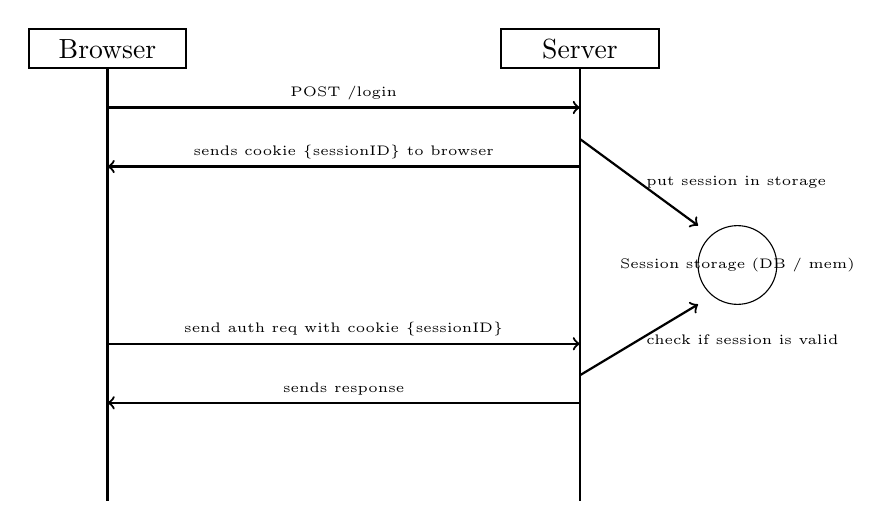
\begin{tikzpicture}

        % Browser entity
        \draw[thick] (0,0) -- node[below] {Browser}
        (2,0) -- (2,-0.5) -- (0,-0.5) -- cycle;

        \draw[thick] (1,-0.5) -- (1,-6);

        % Server entity
        \draw[thick] (6,0) -- node[below] {Server}
        (8,0) -- (8,-0.5) -- (6,-0.5) -- cycle;

        \draw[thick] (7,-0.5) -- (7,-6);


        \tiny
        % DB entity
        \draw (9,-3) circle (0.5cm) node {Session storage (DB / mem)};

        % First request communication
        \draw[->, thick] (1,-1) -- node[above] {POST /login} (7,-1);
        \draw[->, thick] (7,-1.75) -- node[above] {sends cookie \{sessionID\} to browser} (1,-1.75);

        % Second request communication
        \draw[->, thick] (1,-4) -- node[above] {send auth req with cookie \{sessionID\}} (7,-4);
        \draw[->, thick] (7,-4.75) -- node[above] {sends response} (1,-4.75);

        % Server to session storage communication
        \draw[->, thick] (7,-1.4) -- node[right] {put session in storage} (8.5,-2.5);
        \draw[->, thick] (7,-4.4) -- node[right] {check if session is valid} (8.5,-3.5);
    \end{tikzpicture}
\end{frame}

\begin{frame}
    \frametitle{Session based characteristics}

    \begin{itemize}
        \item Easy to implement stateful user sessions
        \item Can revoke at any time
        \item Can store any data alongside your session ID
        \item Can be a bottleneck in case of large volumes / data / traffic
        \item Serialization can be a problem (when storing objects)
        \item Session storage is a bottleneck in distributed contexts
    \end{itemize}

\end{frame}

\begin{frame}
    \frametitle{JWT based}

    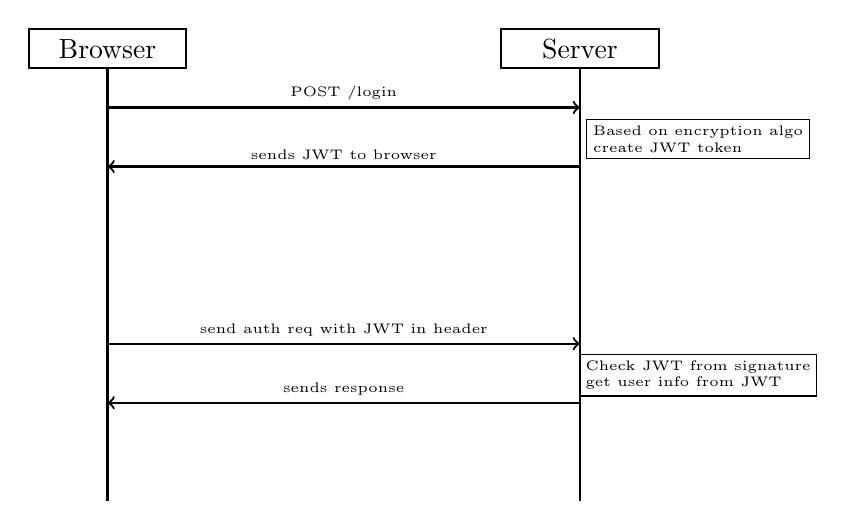
\begin{tikzpicture}
        % Browser entity
        \draw[thick] (0,0) -- node[below] {Browser}
        (2,0) -- (2,-0.5) -- (0,-0.5) -- cycle;

        \draw[thick] (1,-0.5) -- (1,-6);

        % Server entity
        \draw[thick] (6,0) -- node[below] {Server}
        (8,0) -- (8,-0.5) -- (6,-0.5) -- cycle;

        \draw[thick] (7,-0.5) -- (7,-6);

        \tiny
        % First request communication
        \draw[->, thick] (1,-1) -- node[above] {POST /login} (7,-1);
        \draw[->, thick] (7,-1.75) -- node[above] {sends JWT to browser} (1,-1.75);

        % Second request communication
        \draw[->, thick] (1,-4) -- node[above] {send auth req with JWT in header} (7,-4);
        \draw[->, thick] (7,-4.75) -- node[above] {sends response} (1,-4.75);

        % Server operations
        \node[draw,align=left] at (8.5,-1.4) {Based on encryption algo \\ create JWT token};
        \node[draw,align=left] at (8.5,-4.4) {Check JWT from signature \\ get user info from JWT};
    \end{tikzpicture}
\end{frame}

\begin{frame}
    \frametitle{JWT: Where is it exactly?}

    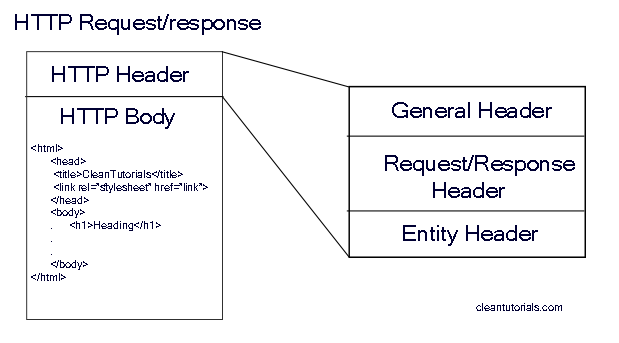
\includegraphics[scale=0.45]{00_http_header.png}
\end{frame}

\begin{frame}
    \frametitle{JWT: What is it exactly?}

    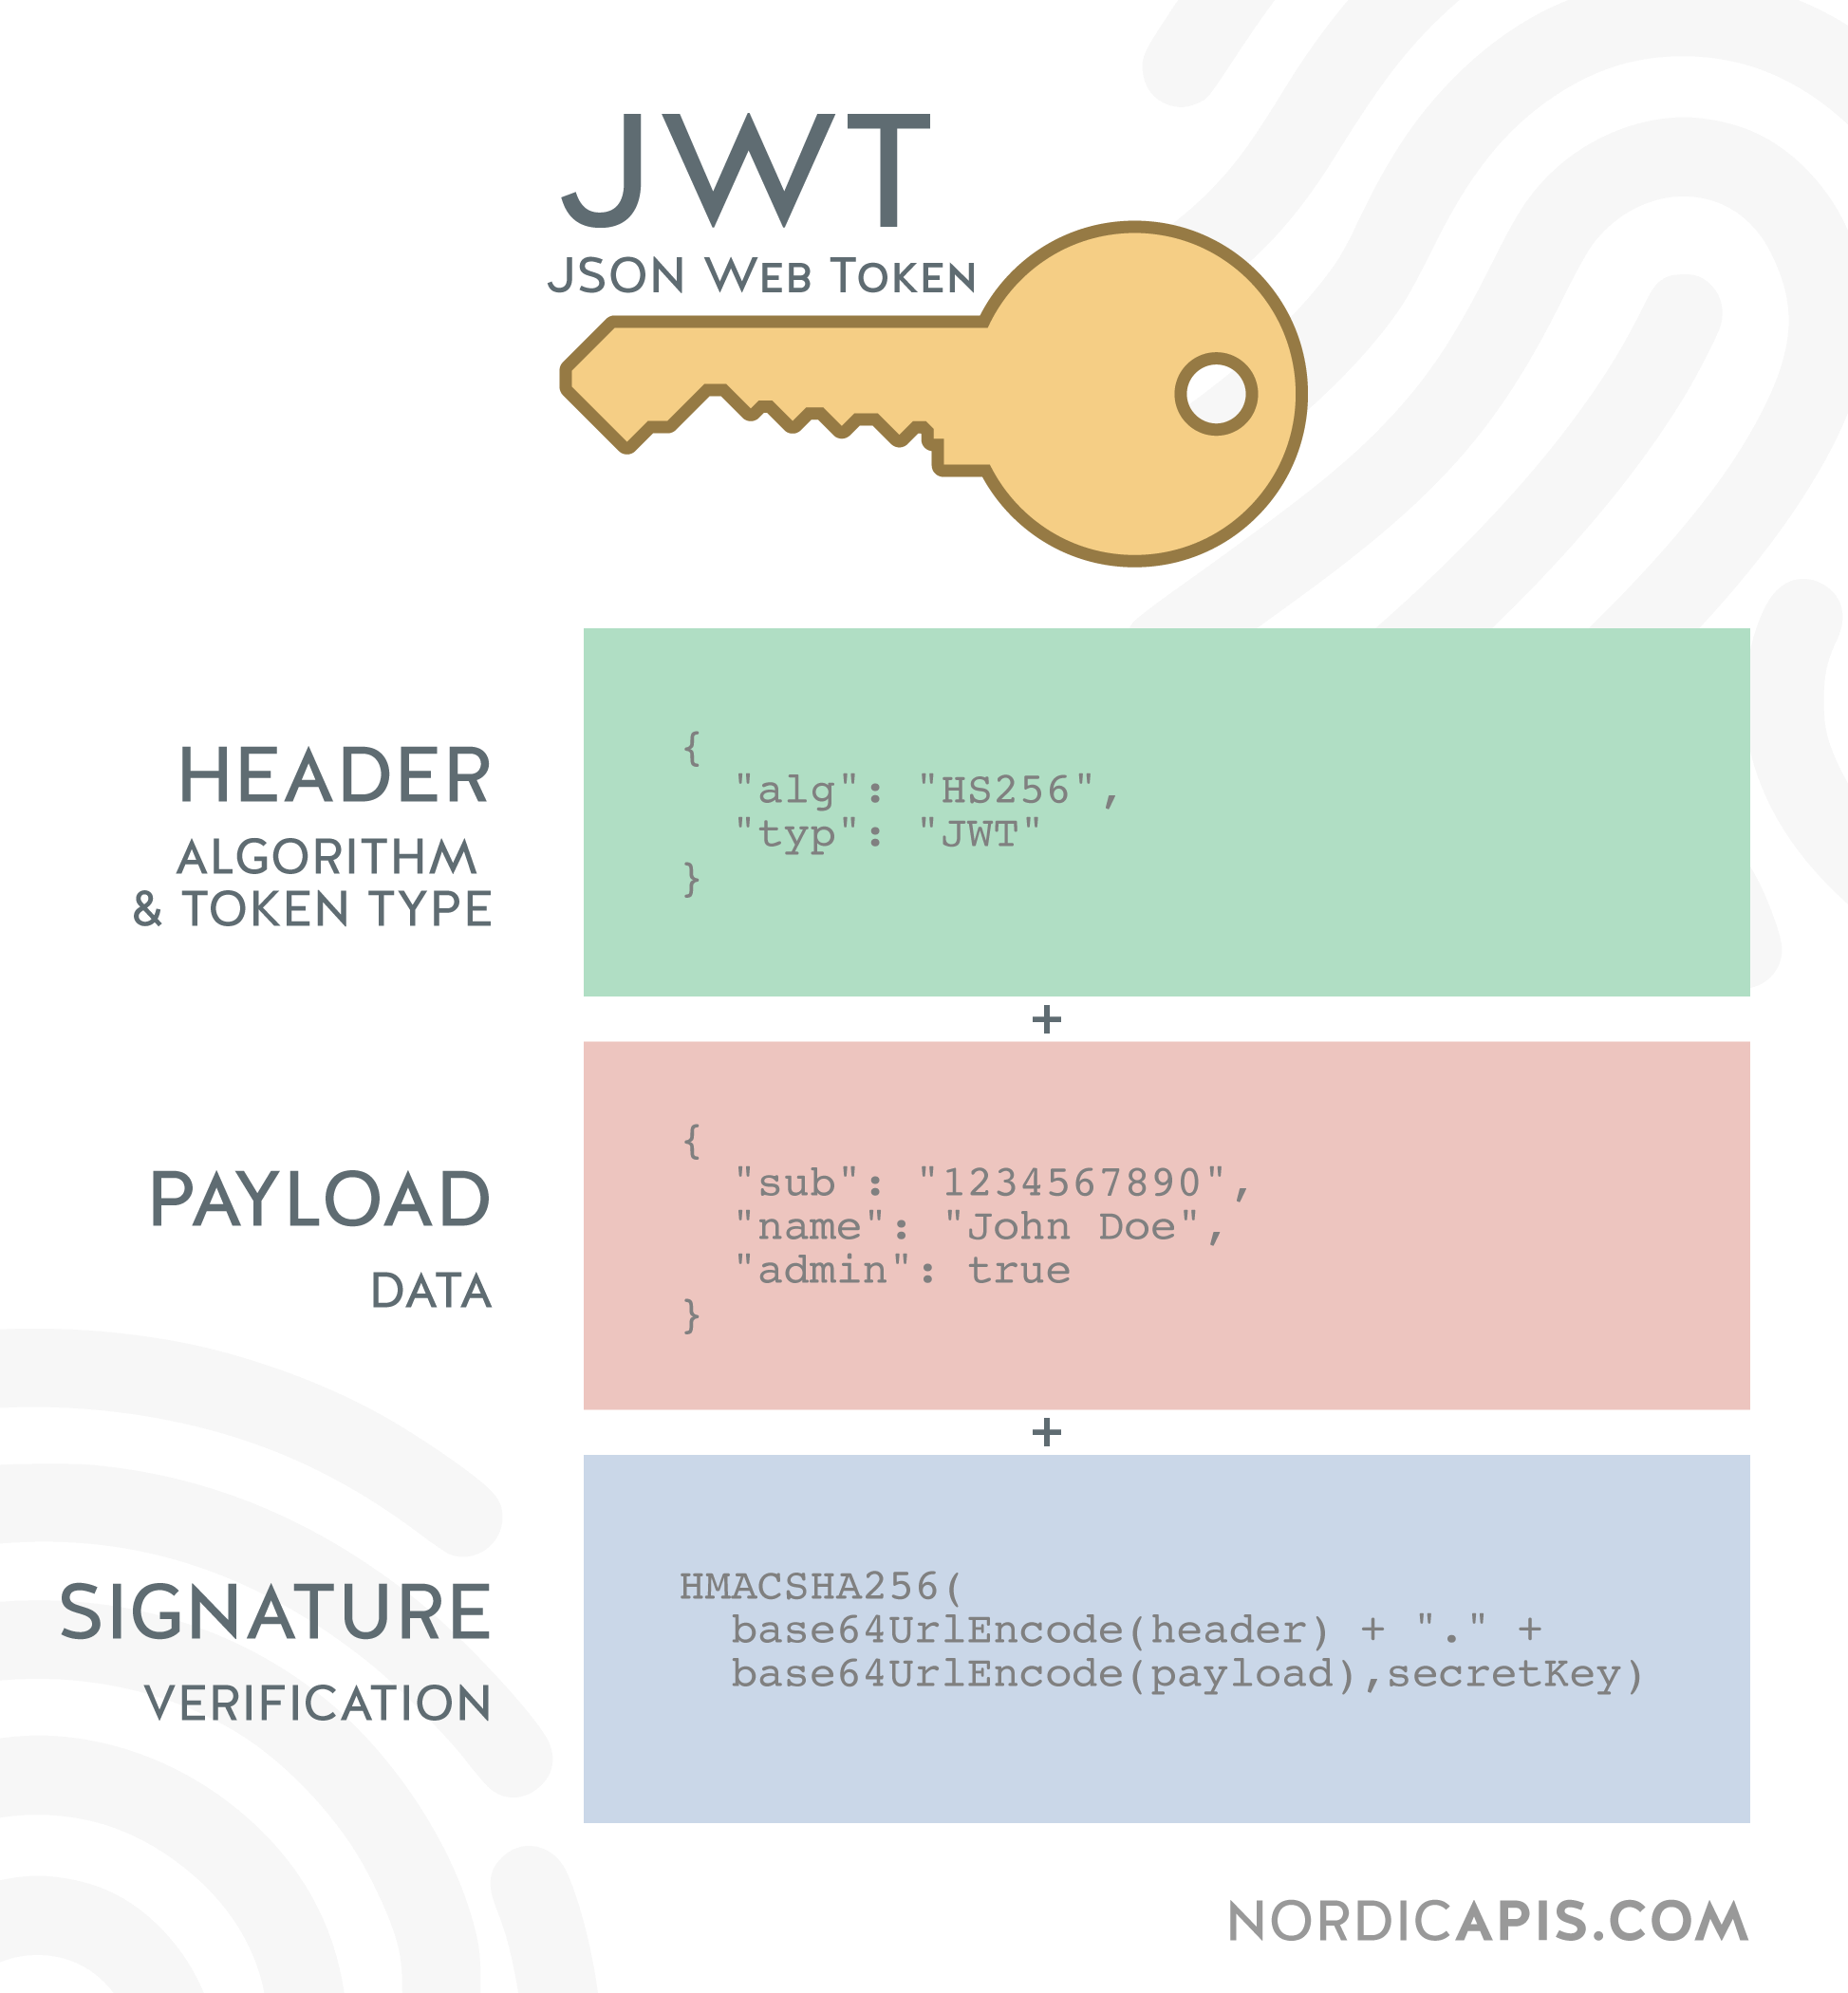
\includegraphics[scale=0.11]{01_jwt.png}
\end{frame}

\begin{frame}
    \frametitle{JWT: What is it exactly?}

    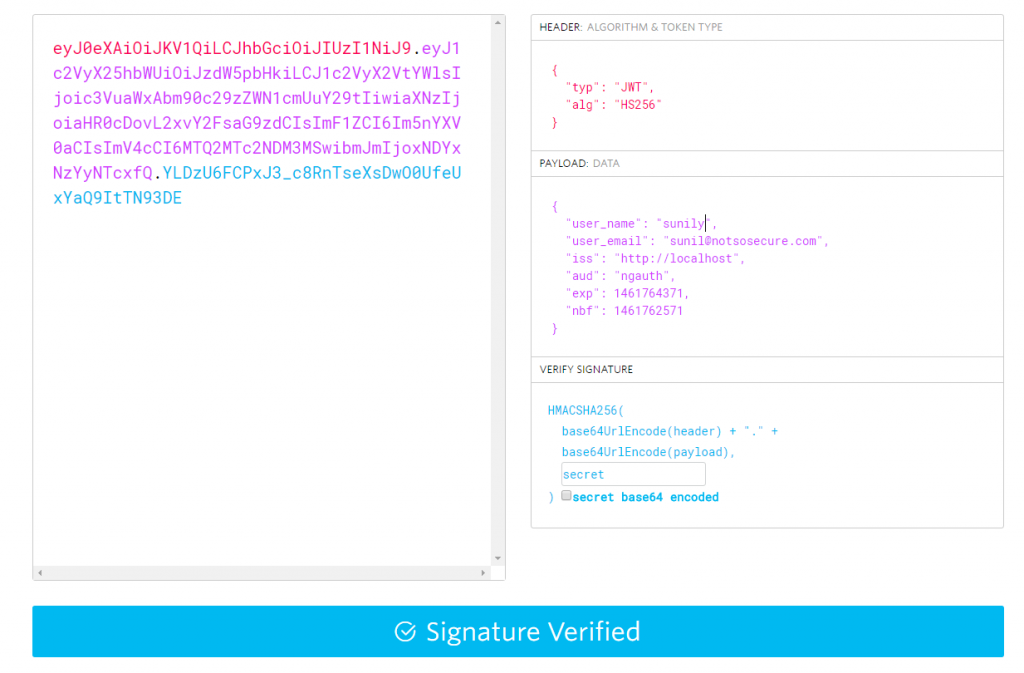
\includegraphics[scale=0.35]{02_jwt.png}
\end{frame}

\begin{frame}
    \frametitle{JWT based characteristics}

    \begin{itemize}
        \item no central bottleneck anymore
        \item allows horizontal scaling
        \item built-in expiration functionality
        \item no way to revoke the JWT token
        \item self-contained, but keep it short
    \end{itemize}
\end{frame}

\begin{frame}
    \frametitle{What to use?}

    \begin{itemize}
        \item Both are viable, depends on your needs
        \item We'll go with JWT (Guardian library) as this can be re-used in Distributed Applications
    \end{itemize}
\end{frame}

\begin{frame}
    \frametitle{Extra references}

    \begin{itemize}
        \item \href{https://medium.com/@sherryhsu/session-vs-token-based-authentication-11a6c5ac45e4}{[LINK]}
        \item \href{https://auth0.com/learn/json-web-tokens/}{[LINK]}
        \item \href{https://medium.com/@theflyingmantis/session-vs-jwt-token-based-authentication-2e85ff6c8f42}{[LINK]}
        \item \href{https://ponyfoo.com/articles/json-web-tokens-vs-session-cookies}{[LINK]}
        \item \href{https://www.pingidentity.com/fr/company/blog/posts/2019/the-hard-parts-of-jwt-security-nobody-talks-about.html}{[LINK]}
        \item \href{https://stormpath.com/blog/where-to-store-your-jwts-cookies-vs-html5-web-storage}{[LINK STORAGE]}
        \item \href{https://www.jsonwebtoken.io/}{[LINK VERIFY MANUALLY]}
    \end{itemize}
\end{frame}
